% \documentclass{book}

\documentclass[12pt]{article}
\usepackage[pdfborder={0 0 0.5 [3 2]}]{hyperref}%
\usepackage[left=1in,right=1in,top=1in,bottom=1in]{geometry}%
\usepackage[shortalphabetic]{amsrefs}%
\usepackage{amsmath}
\usepackage{enumerate}
\usepackage{enumitem}
\usepackage{amssymb}                
\usepackage{amsmath}                
\usepackage{amsfonts}
\usepackage{amsthm}
\usepackage{bbm}
\usepackage[table,xcdraw]{xcolor}
\usepackage{tikz}
\usepackage{float}
\usepackage{booktabs}
\usepackage{svg}
\usepackage{mathtools}
\usepackage{cool}
\usepackage{url}
\usepackage{graphicx,epsfig}
\usepackage{hyperref}  

\usetikzlibrary{automata,arrows,positioning,calc}
\DeclarePairedDelimiter\abs{\lvert}{\rvert}%
\DeclarePairedDelimiter\norm{\lVert}{\rVert}%
\DeclarePairedDelimiter\ceil{\lceil}{\rceil}
\DeclarePairedDelimiter\floor{\lfloor}{\rfloor}

\makeatletter
\renewcommand*\env@matrix[1][*\c@MaxMatrixCols c]{%
  \hskip -\arraycolsep
  \let\@ifnextchar\new@ifnextchar
  \array{#1}}
\makeatother

\newtheorem{theorem}{Theorem}[section]
\newtheorem{corollary}{Corollary}[theorem]
\newtheorem{proposition}[theorem]{Proposition}
\newtheorem{lemma}[theorem]{Lemma}

\theoremstyle{definition}
\newtheorem{definition}[theorem]{Definition}
\newtheorem{exercise}{Exercise}%
\newtheorem{problem}[exercise]{Problem}%
\newtheorem*{example}{Example}

\theoremstyle{remark}
\newtheorem*{question}{Question}
\newtheorem*{observation}{Observation}
\newtheorem*{remark}{Remark}

\graphicspath{ {images/} }

\setlength{\parindent}{0cm}
\renewcommand{\vec}[1]{\ensuremath{\mathbf{#1}}}

\def\noi{\noindent}
\def\T{{\mathbb T}}
\def\R{{\mathbb R}}
\def\N{{\mathbb N}}
\def\C{{\mathbb C}}
\def\Z{{\mathbb Z}}
\def\P{{\mathbb P}}
\def\E{{\mathbb E}}
\def\Q{\mathbb{Q}}
\def\ind{{\mathbb I}}

\def\cale{{\mathcal E}}
\def\cals{{\mathcal S}}
\def\calc{{\mathcal C}}
\def\caln{{\mathcal N}}
\def\calb{{\mathcal B}}
\def\calg{{\cal G}}

\def\ds{\displaystyle}
\def\ra{\rightarrow}
\newcommand{\conv}{\mbox{\rm conv}}
\newcommand{\spaan}{\mbox{\rm span}}
\newcommand{\deet}{\mbox{\rm det}}
\newcommand{\aff}{\mbox{\rm aff}}
\newcommand{\cl}{\mbox{\rm cl}}
\newcommand{\dimm}{\mbox{\rm dim}}
\newcommand{\sm}{\setminus}
\def\ci{\perp\!\!\!\perp}


\newcommand{\ink}{\rule{.5\baselineskip}{.55\baselineskip}}

\begin{document}

\section{Probability}
In general parlance, the term \emph{probability} is used as a measure of a person's belief in the occurrence of a future event. Take a sentence such as, ``There is a 50\% probability of rain tomorrow''. A professional meteorologist has used a sophisticated mathematical model to distill large amounts of atmospheric data down to a simple number indicating her belief that it is equally likely to rain or not rain tomorrow. We can intepret this number however we wish. Who does this meterologist work for? How reliable have their predictions been in the past? (Here, we should examine our biases, for we might be more likely to recall rain when none was predicted than the other way around.) Then we can use this number to make decisions such as whether or not to carry an umbrella.\\

We can put this idea on a more mathematical footing by looking at the \emph{empirical probability} (or relative frequency) of an event. Imaging rolling a standard six-sided die repeatedly. The empirical probability of rolling a 1 is the ratio of the number of times a 1 is rolled to the total number of rolls. In general, we have:
\[
\text{empirical probability of a certain event} = \frac{ \text{number of times the event occurs }}{\text{total number of trials}}
\]
Intuitively, as we perform more and more dice rolls, the empirical probability of rolling a 1 should approach some mythical quantity which we call the \emph{probability} of rolling a 1. Using a symmetry argument, since dice are cubical and there should be no reason for one face to be preferred over another, this probability should be 1/6. This idea, which is known as the \emph{law of large numbers} will be made rigorous later in the course.\\

For now, however, we require a more rigorous, mathematical definition of probability, and for that we turn to the language of \emph{set theory}.

\subsection{Sample Spaces}
A \emph{set} is a collection of distinct objects. A \emph{sample space}, denoted $\cals$ is the set of all outcomes of a particular experiment. Here are some examples of sample spaces:
\begin{enumerate}
\item Single coin flip: $\cals = \{H, T\}$
\item Roll of one standard, six-sided die: $\cals = \{1, 2, 3, 4, 5, 6\}$
\item Roll of two standard, six-sided dice: Here we represent the sample spaces as ordered pairs.

\begin{figure}[H]
\centering
% \caption{My caption}
\label{twodice}
\begin{tabular}{llllllll}
           &                        &        &        & \multicolumn{2}{l}{second roll} &        &                             \\
           &                        & 1      & 2      & 3              & 4              & 5      & 6                           \\ \cline{3-8} 
           & \multicolumn{1}{l|}{1} & (1, 1) & (1, 2) & (1, 3)         & (1, 4)         & (1, 5) & \multicolumn{1}{l|}{(1, 6)} \\
           & \multicolumn{1}{l|}{2} & (2, 1) & (2, 2) & (2, 3)         & (2, 4)         & (2, 5) & \multicolumn{1}{l|}{(2, 6)} \\
first roll & \multicolumn{1}{l|}{3} & (3, 1) & (3, 2) & (3, 3)         & (3, 4)         & (3, 5) & \multicolumn{1}{l|}{(3, 6)} \\
           & \multicolumn{1}{l|}{4} & (4, 1) & (4, 2) & (4, 3)         & (4, 4)         & (4, 5) & \multicolumn{1}{l|}{(4, 6)} \\
           & \multicolumn{1}{l|}{5} & (5, 1) & (5, 2) & (5, 3)         & (5, 4)         & (5, 5) & \multicolumn{1}{l|}{(5, 6)} \\
           & \multicolumn{1}{l|}{6} & (6, 1) & (6, 2) & (6, 3)         & (6, 4)         & (6, 5) & \multicolumn{1}{l|}{(6, 6)} \\ \cline{3-8} 
\end{tabular}
\end{figure}

\item Number of free throw attempts it takes for me to make a single basket: $\cals = \{1, 2, 3, ...\}$. This set is often denoted $\N$ for the natural numbers (positive integers)
\item Number of minutes late my RIPTA bus arrives: $\cals = [0, \infty)$. 
\end{enumerate}
Note that the first three sample spaces contain only a finite number of elements (2, 6, and 36 elements, respectively). These are called \emph{finite sample spaces}. The fourth and fifth sample spaces both contain an infinite number of elements, but there is a fundamental difference between the two. The set $\N$ can be written out in its entirety in an infinitely long list; another way to think about this is that we can start at 1 and count up to any number in the set (as long as we have enough time!). A set with this property is called \emph{countable}. For the set $[0, \infty)$, it makes intuitive sense that we cannot do this, i.e. we cannot list all the elements and, say, ``count up to $\pi$''. A proof of this fact is left for another course. Such an infinite set is called \emph{uncountable}\footnote{An uncountable set is a ``larger infinity'' than a countable set, which leads to the concept of ``sizes of infinity''. John Green alludes to this in his novel \emph{The Fault in Our Stars}, but unforunately gets the math wrong. If you find this interesting, I recommend the Vi Hart video \url{https://www.youtube.com/watch?v=23I5GS4JiDg}}. A sample space which is either finite or countable is called \emph{discrete}.\\

\subsection{Events and Subsets}
An \emph{event} is a subset of a sample space. Events are usually designated by capital letters, and we write the relationship ``$A$ is a subset of $\cals$'' by $A \subset \cals$. For two events $A$ and $B$, $A \subset B$ if every element in $A$ is also contained in $B$. The \emph{empty set}, denoted $\emptyset$, is the set containing no elements, and it is a subset of every set.
\\

Let us consider the sample space $\cals = \{1, 2, 3, 4, 5, 6\}$, representing the roll of a single die. The following are examples of events:
\begin{enumerate}
\item $A = \{2, 4, 6\}$, the event that an even number is rolled
\item $B = \{1, 2, 3\}$, the event that the roll is less than or equal to 3
\item $C = \{1\}$, the event that a 1 is rolled
\end{enumerate}
The event $C$ consists of a single element in the sample space. Such an event is called a \emph{simple event} and cannot be decomposed. The events $A$ and $B$ are each composed of three simple events.\\

Next, consider the sample space repesenting rolls of two dice. Let $E$ be the event that the sum of the two dice is 7. We can represent this event graphically; in the figure below, the event $E$ consists of the squares which are highlighted in yellow.

% Please add the following required packages to your document preamble:
% \usepackage[table,xcdraw]{xcolor}
% If you use beamer only pass "xcolor=table" option, i.e. \documentclass[xcolor=table]{beamer}
\begin{figure}[H]
\centering
% \caption{My caption}
\label{two-dice-sum-seven}
\begin{tabular}{llllllll}
           &                        &                                                     &                                                     & \multicolumn{2}{l}{second roll}                                                                           &                                                     &                                                     \\
           &                        & 1                                                   & 2                                                   & 3                                                   & 4                                                   & 5                                                   & 6                                                   \\ \cline{3-8} 
           & \multicolumn{1}{l|}{1} & (1, 1)                                              & (1, 2)                                              & (1, 3)                                              & (1, 4)                                              & \multicolumn{1}{l|}{(1, 5)}                         & \multicolumn{1}{l|}{\cellcolor[HTML]{F8FF00}(1, 6)} \\ \cline{7-8} 
           & \multicolumn{1}{l|}{2} & (2, 1)                                              & (2, 2)                                              & (2, 3)                                              & \multicolumn{1}{l|}{(2, 4)}                         & \multicolumn{1}{l|}{\cellcolor[HTML]{F8FF00}(2, 5)} & \multicolumn{1}{l|}{(2, 6)}                         \\ \cline{6-7}
first roll & \multicolumn{1}{l|}{3} & (3, 1)                                              & (3, 2)                                              & \multicolumn{1}{l|}{(3, 3)}                         & \multicolumn{1}{l|}{\cellcolor[HTML]{F8FF00}(3, 4)} & (3, 5)                                              & \multicolumn{1}{l|}{(3, 6)}                         \\ \cline{5-6}
           & \multicolumn{1}{l|}{4} & (4, 1)                                              & \multicolumn{1}{l|}{(4, 2)}                         & \multicolumn{1}{l|}{\cellcolor[HTML]{F8FF00}(4, 3)} & (4, 4)                                              & (4, 5)                                              & \multicolumn{1}{l|}{(4, 6)}                         \\ \cline{4-5}
           & \multicolumn{1}{l|}{5} & \multicolumn{1}{l|}{(5, 1)}                         & \multicolumn{1}{l|}{\cellcolor[HTML]{F8FF00}(5, 2)} & (5, 3)                                              & (5, 4)                                              & (5, 5)                                              & \multicolumn{1}{l|}{(5, 6)}                         \\ \cline{3-4}
           & \multicolumn{1}{l|}{6} & \multicolumn{1}{l|}{\cellcolor[HTML]{F8FF00}(6, 1)} & (6, 2)                                              & (6, 3)                                              & (6, 4)                                              & (6, 5)                                              & \multicolumn{1}{l|}{(6, 6)}                         \\ \cline{3-8} 
\end{tabular}
\end{figure}

\subsection{Basic Set Operations}
Let $\cals$ be our sample space, the set of all elements under consideration. Consider two events $A$ and $B$ which are subsets of $\cals$. We have the following three basic set operations, which are handily illustrated using Venn diagrams.
\begin{enumerate}
\item The \emph{union} of $A$ and $B$, denoted $A \cup B$, is the set of all elements which are in $A$ or $B$ (or both). That is, the union is all elements that are in at least one of the two sets.
\begin{figure}[H]
\centering
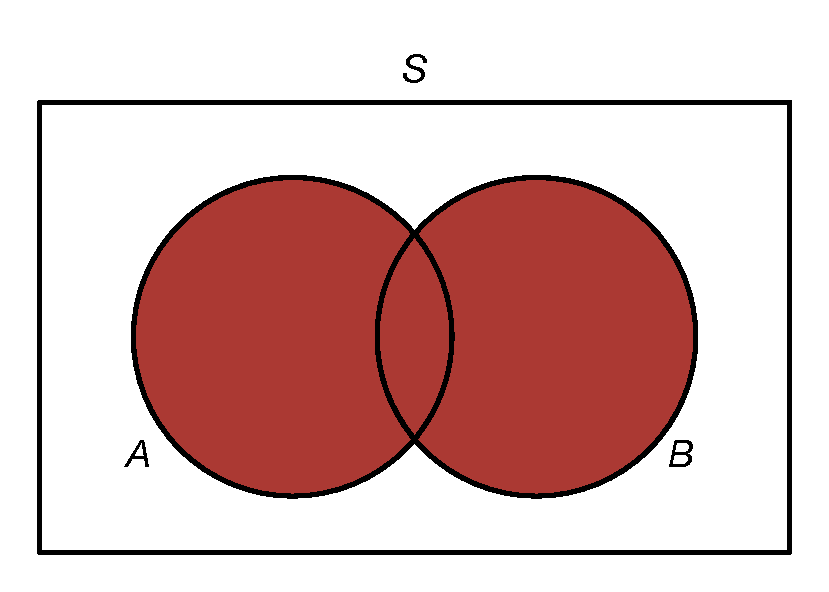
\includegraphics[width=8cm]{AunionB}
\end{figure}
\item The \emph{intersection} of $A$ and $B$, denoted $A \cap B$, is the set of all elements which are in both $A$ and $B$.
\begin{figure}[H]
\centering
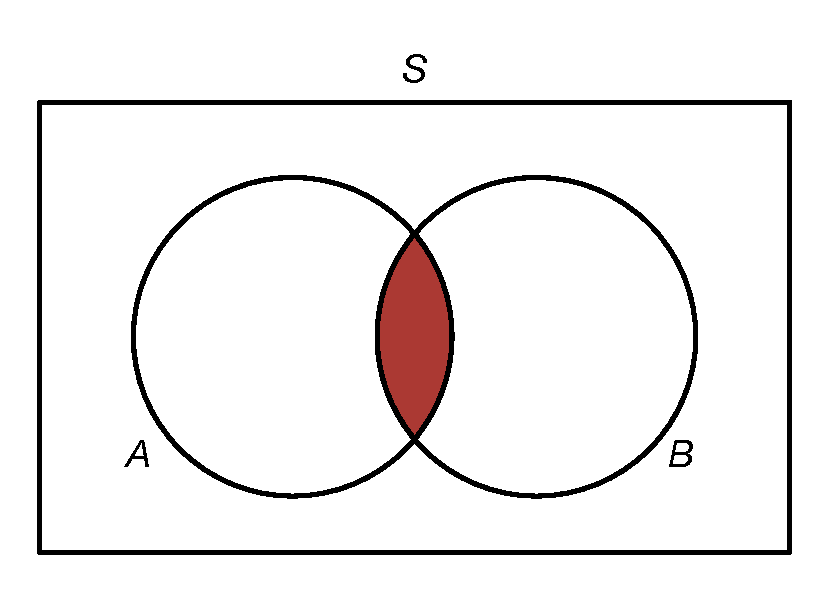
\includegraphics[width=8cm]{AintersectB}
\end{figure}
Two sets $A$ and $B$ are \emph{disjoint} or \emph{mutually exclusive} if they have no elements in common, i.e. if $A \cap B = \emptyset$.
\begin{figure}[H]
\centering
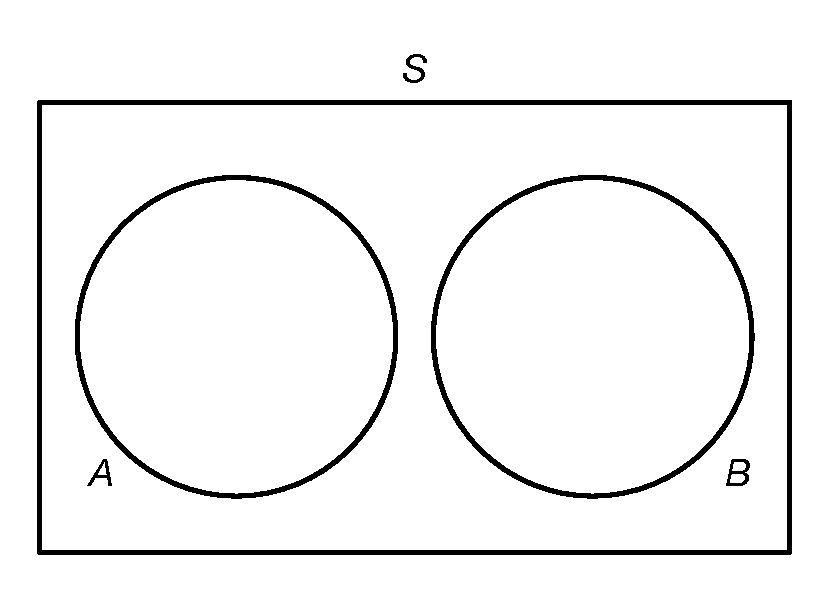
\includegraphics[width=8cm]{exclusive}
\end{figure}
\item The \emph{complement} of $A$, denoted $A^c$, is the set of all points in $\cals$ which are not in $A$. Note that $A$ and $A^c$ are disjoint, and $A \cup A^c = \cals$.
\begin{figure}[H]
\centering
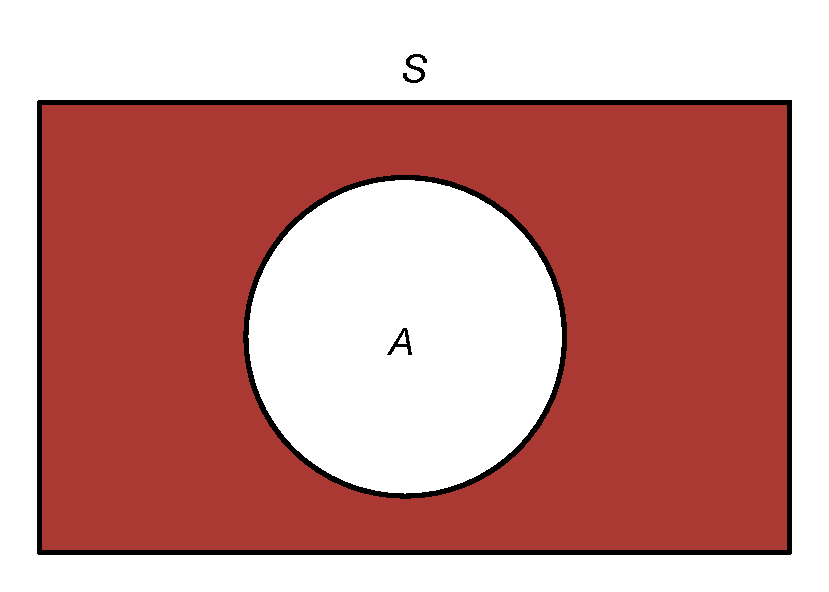
\includegraphics[width=8cm]{Acomplement}
\end{figure}
\end{enumerate}
There are many relationships between these operations which fall under the rubric of set algebra. Most of them we will not need, but we mention a few useful ones here:
\begin{enumerate}
\item Distributive laws
\begin{align*}
A \cap (B \cup C) &= (A \cap B) \cup (A \cap C) \\
A \cup (B \cap C) &= (A \cup B) \cap (A \cup C)
\end{align*}
\item DeMorgan's laws
\begin{align*}
(A \cap B)^c &= A^c \cup B^c &\text{(the complement of an intersection is the union of the complements)}\\
(A \cup B)^c &= A^c \cap B^c &\text{(the complement of a union is the intersection of the complements)}
\end{align*}
\end{enumerate}

\subsection{Axiomatic Definition of Probability}
Equipped with our our knowlege of set theory, we can define probability axiomatically as follows. Given any event $A$ in our sample space $\cals$, we assign a probability $\P(A)$ to that event such that the following rules hold:
\begin{enumerate}
\item $0 \leq \P(A) \leq 1$ \\

The probability of an event is a real number between 0 and 1, where a probability of 0 means that the event will never occur, and a probability of 1 means that the event will always occur.
\item $\P(\emptyset) = 0$ \\

The probability that nothing happens is 0, i.e. something must happen.
\item $\P(\cals) = 1$ \\

The probability of the whole sample space is 1, which is another way of saying that something must happen.
\item If $A \subset B$, then $\P(A) \leq \P(B)$ \\

If we make a set bigger, its probability can only increase (or stay the same); it cannot decrease.

\item If $A_1, A_2, \dots, A_n$ are pairwise disjoint events, i.e. $A_i \cap A_j = \emptyset$ if $i \neq j$, then
\[
\P(A_1 \cup A_2 \cup \cdots \cup A_n) = \sum_{i=1}^n \P(A_i)
\]
This holds for an infinite sequence as well, i.e. if $A_1, A_2, A_3, \dots$ are a sequence of pairwise disjoint events, then 
\[
\P(A_1 \cup A_2 \cup A_3 \cup \cdots) = \sum_{i=1}^\infty \P(A_i)
\]
\end{enumerate}

From these we can derive a very important rule:
\[
\P(A) + \P(A^c) = 1, \:\:\text{ i.e. }\P(A) = 1 - \P(A^c)
\]
Sometimes it is easier to calculate the probability of an event \emph{not} happening than the probability of the event itself!\\

These rules tell us the properties that we want probability to have. However, given a sample space, they do not actually tell us how to assign probabilities to each event in the sample space. Doing that in a way that is consistent with the above rules can be a bit tricky \footnote{In fact, for an uncountable sample space such as $\cals = [0, 1]$, you can show that you cannot construtct a notion of probability which is consistent with all the rules; this is the starting point for the development of measure theory, and is beyond the scope of this course.}, but luckily for a discrete sample space we can do this with no problem. Since a discrete sample space is composed of a finite (or countable) number of simple events, all we have to do is assign probabilities to each simple event in such a way that they all add up to 1.

\begin{example}Consider once again tossing a single die. The sample space for this is $\cals = \{1, 2, 3, 4, 5, 6\}$. This sample space contains 6 simple events: $\{1\}, \{2\}, \{3\},\{4\}, \{5\}$, and $\{6\}$. We can assign any probabilties we want to these simple events, as long as they add up to 1. For example, assuming we have a fair die, we can let $\P(\{i\}) = 1/6$ for $i = 1, \dots, 6$. If we like, we can check that all the above rules hold. If we have a loaded die, which rolls a 6, say, half the time, we could assign probabilites: $\P(\{6\}) = 1/2, \P(\{i\}) = 1/10$ for $i = 1, \dots, 5$.
\end{example}

\begin{example}Consider this time a countable sample space $\cals = \N = \{1, 2, 3, \dots\}$. One possibility is to assign probabilities $\P(\{i\}) = 1/2^i$ for $i = 1, 2, 3, \dots$, i.e. $\P(\{1\}) = 1/2$, $\P(\{2\}) = 1/4$, $\P(\{3\}) = 1/8$, etc. Perhaps you recall from calculus that this is a geometric series, and so we know its sum is:
\[
\sum_{i = 1}^{\infty} \P(\{i\}) = \sum_{i = 1}^{\infty} \frac{1}{2^i} = \frac{1}{2}\frac{1}{1 - 1/2} = 1
\]
Since the sum of the probabilities of all the simple events is 1, we are all set! If you have not seen this before, we will cover this in more detail when we discuss the geometric distribution. In the meantime, here is a nice picture to convince you that the sum is indeeed 1.
\begin{figure}[H]
\centering
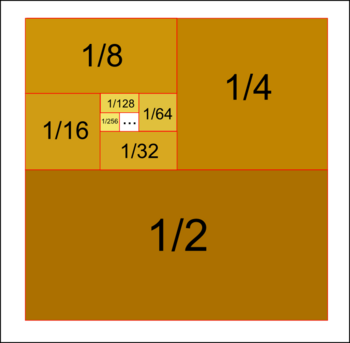
\includegraphics[width=5cm]{Geometric_series}
\end{figure}
\end{example}

\subsection{Discrete Uniform Distribution}
The first probability distribution we will consider is the uniform distribution on a \emph{finite} sample space. In the discrete uniform distribution, every simple event is equally likely to occur. If we have a finite sample space with $n$ simple events, then the discrete uniform distribution assigns each simple event a probability of $1/n$.

\begin{example}Consider the finite sample space $\cals$ representing the roll of two standard dice. This sample space has 36 simple events, so each simple event has a probability of 1/36. Note that for the simple events in this sample space, the order of the die rolls matters. $(1, 6)$ and $(6, 1)$ are two different eventsl; even though both events contain the same die rolls, for the former, the 1 is rolled first, while for the latter, the 6 is rolled first.
\begin{enumerate}
\item What is the probability that the sum of the two dice is 7? Looking at the graphical depiction of this event above, we see that there are 6 simple events that give us a sum of 7. Thus the probability of a sum of 7 is 6/36 = 1/6.
\item What is the probability that the sum of the two dice is less than 11. In this case, it is easier to compute the probability that the sum is 11 or greater and then subtract that probability from 1. (Why can we do this?) Let $A$ be the event that the sum is 11 or greater. $A$ is composed of 3 simple events: $(6, 6), (6, 5)$, and $(5, 6)$. Thus we have $\P(A) = 3/36$. The probability we want is:
\[
\P(A^c) = 1 - \P(A) = 1 - 3/36 = 33/36
\]
\end{enumerate}
\end{example}
In the previous example, it is relatively straightforward to draw the sample space, so we can essentially compute any probabily we want simply by looking at the picture and counting which boxes comprise our event of interest. For more complicated problems, this is not as easy. Consider the following example:

\begin{example}A communication system consists of $n$ antennas arranged in a line. Exactly $m$ out of the $n$ antennas are defective. The system is functional if no two consecutive antennas are defective. Assuming that each linear arrangement of the antennas is equally likely, what is the probability that the system will be functional?\\

For small values of $n$ and $m$, say $n = 4$ and $m = 2$, we can write out all of the possible configurations. Representing a functional antenna by 1 and a defective antenna by 0, there are exactly six linear arrangements:
\begin{enumerate}[noitemsep]
\item 0 1 1 0
\item 0 1 0 1
\item 0 0 1 1
\item 1 0 0 1
\item 1 0 1 0
\item 1 1 0 0
\end{enumerate}
Take a moment to convince yourself that these are the only possible configurations. Configurations 1, 2, and 5 are functional, so there are 3 functional configurations out of 6 total configurations. So in this case, the probability that the system is functional is 3/6. \\

For general $n$ and $m$, it is not immediately obvious how to perform the requisite counting of configurations. Taking a cue from the Count on Sesame Street, we need to learn more about counting. The mathematical theory of counting is known as \emph{combinatorics}.
\end{example}

\subsubsection{The Basic Principle of Counting}

We have already seen the \emph{basic principle of counting} in play when we looked at the sample space for two dice. 


\subsubsection{Permutations}

\subsubsection{Combinations}

\subsubsection{}


\subsubsection{Multinomials}

\end{document}
